%% Example data sheet
%% Feel free to modify and use this file for any purpose, under
%% either the LaTeX Project Public License or under public domain.

% Options here are passed to the article class.
% Most common options: 10pt, 11pt, 12pt

\documentclass[10pt]{datasheet}

% Input encoding and typographical rules for English language
\usepackage[utf8]{inputenc}
\usepackage[english]{babel}
\usepackage[english]{isodate}

% tikz is used to draw images in this example, but you can
% also use \includegraphics{}.
\usepackage{tikz}
\usepackage{pgfplots}
\usepackage{circuitikz}
\usetikzlibrary{calc}

% These define global texts that are used in headers and titles.
\title{OBC v1.2 Datasheet}
\author{UTAT Space Systems}
\date{May 2025}
\revision{Revision 1}
\companylogo{
\includegraphics[scale=0.022]{figures/utat_ss.png}}
\usepackage[super,square]{natbib}
\usepackage{anysize}
\usepackage{graphicx} 
\marginsize{1.5cm}{1.5cm}{1cm}{1cm}
\usepackage{fancyhdr}
\renewcommand{\headrulewidth}{0pt}
\usepackage[dvipsnames]{xcolor}
\usepackage{hyperref}
\hypersetup{
    colorlinks=true,
    linkcolor=black,
    citecolor=CadetBlue,
    filecolor=CadetBlue,      
    urlcolor=CadetBlue,
}
\usepackage{multicol}
\setlength\columnsep{18pt}
\renewenvironment{abstract}
 {\par\noindent\textbf{\abstractname}\ \ignorespaces \\}
 {\par\noindent\medskip}
\renewcommand*{\thefootnote}{\fnsymbol{footnote}}
\usepackage{amsmath}


\usepackage{xcolor}
\usepackage{comment}
\usepackage{multirow}
\usepackage{float}
\usepackage{gensymb}
\usepackage{braket}
\usepackage{longtable}
\usepackage{caption}
\usepackage{longtable}
\usepackage{physics}
\usepackage{amsthm}
\usepackage{amsmath}
\usepackage{amssymb}
\usepackage{xcolor}
\usepackage{soul}
\usepackage{ marvosym }
\usepackage{wasysym}
\usepackage [autostyle, english = american]{csquotes}
\usepackage{fancyheadings}
\usepackage{enumitem}
\usepackage{multicol}


\MakeOuterQuote{"}

\newcommand{\xhat}{\hat{\vb x}}
\newcommand{\yhat}{\hat{\vb y}}
\newcommand{\zhat}{\hat{\vb z}}
\newcommand{\nhat}{\hat{\vb n}}
\newcommand{\rhat}{\hat{\vb r}}
\newcommand{\thetahat}{\hat{\vb \theta}}
\newcommand{\phihat}{\hat{\vb \phi}}


\renewcommand{\a}{\alpha}
\renewcommand{\b}{\beta}
\newcommand{\g}{\gamma}
\renewcommand{\d}{\delta}
\newcommand{\e}{\varepsilon}
\renewcommand{\l}{\lambda}
\renewcommand{\t}{\tau}
\newcommand{\w}{\omega}
\newcommand{\A}{\Alpha}
\newcommand{\B}{\Beta}
\newcommand{\G}{\Gamma}
\newcommand{\D}{\Delta}
\newcommand{\W}{\Omega}

\newcommand{\R}{\mathbb{R}}





\begin{document}
\maketitle

\section{Features}

\begin{itemize}
  \item{Features an STM32G431RBT6 MCU}
        \begin{description}
          \item[-] ARM Cortex-M4
          \item[-] 128 kBytes of Flash
          \item[-] LQFP-64 Package
        \end{description}
  \item{HSE: 24MHz. LSE: 32.768kHz}
  \item{}
\end{itemize}



\section{General Description}
The \textbf{datasheet} document class makes it easy to write great looking
data sheets using the LaTeX typesetting system. It follows the classic style used
by most manufacturers of electronic components.

You can download the document class from
\href{https://github.com/PetteriAimonen/latex-datasheet-template/}{latex-datasheet-template}
GitHub repository.
The repository includes this example datasheet as \textbf{example.tex} and
the document class as \textbf{datasheet.cls}.
You can build the PDF document using command \texttt{latexmk -pdf}.

% Switch to next column
\vfill\break

% \begin{figure}[h]
%     \begin{circuitikz}[european]
%         \node[op amp] (amp1) {};
%         \node[op amp, below = 0.5cm, xscale = -1] (amp2) {};
%         \draw (amp1.out) |- (amp2.-);
%         \draw (amp2.-) ++(0, 0.3cm) node[circ]{} to +(2,0) node[above left]{5};
%         \draw (amp2.out) to (amp1.+);
%         \draw (amp1.+) ++(0, -0.3cm) node[circ]{} to +(-2,0) node[above right]{2};
%         \draw (amp1.-) to +(-2,0) node[above right]{1};
%         \draw (amp2.+) to +(2,0) node[above left]{4};
%         \draw (amp1.out) +(0,0.5cm) node (Vdd) {$\mathrm{V_{DD}}$};
%         \draw (Vdd.east) to +(1.5,0) node [above left]{6};
%         \draw (amp2.out) +(0,-0.5cm) node (Vss) {$\mathrm{V_{SS}}$};
%         \draw (Vss.west) to +(-1.6,0) node [above right]{3};
%         \draw ($(amp1.north west) + (-0.5,0.5)$) rectangle ($(amp2.south west) + (0.5,-0.5)$);
%     \end{circuitikz}
%     \caption{Pinout and internal circuit}
% \end{figure}

\begin{figure}[H]
  \centering
  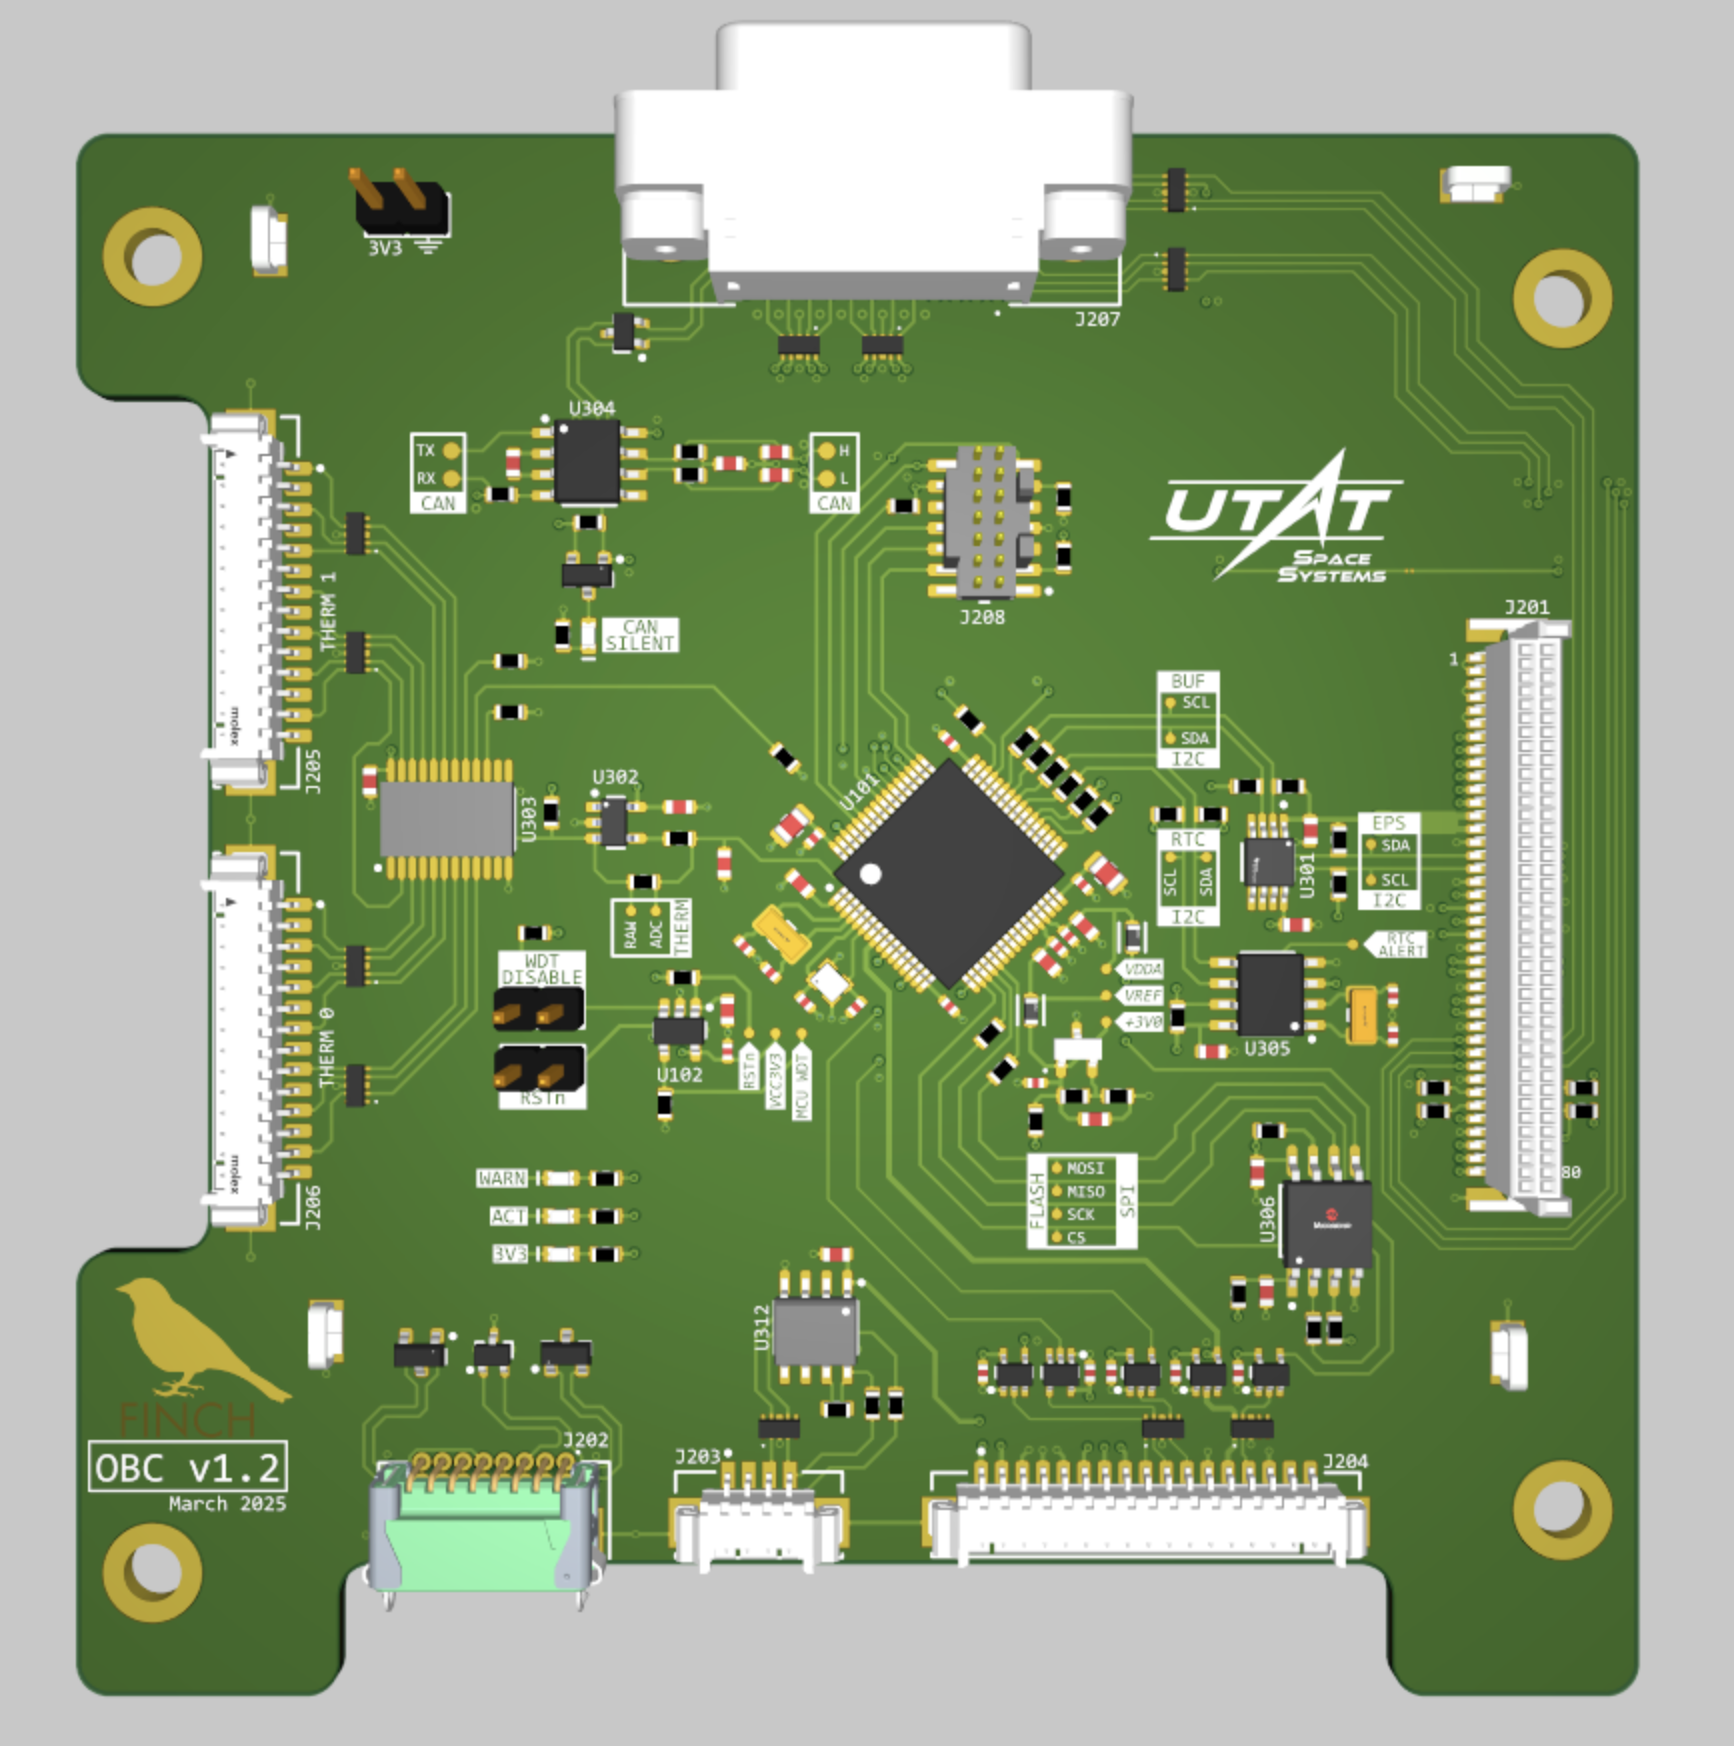
\includegraphics[width=0.95\linewidth]{figures/OBC_SS.png}
  \caption{\centering OBC v1.2}
  \label{fig:enter-label}
\end{figure}

% For wide tables, a single column layout is better. It can be switched
% page-by-page.
\onecolumn
\section{Block Diagram}

\section{Electrical Specifications}
\section{Board Layout}
\section{Timing}
\section{Peripherals}
\section{Sensors}
\subsection{Thermistors}
\section{Manufacturing}
\end{document}

